\section{Værktøjer}
\begin{wrapfigure}{r}{0.3\textwidth}
  \begin{center}
    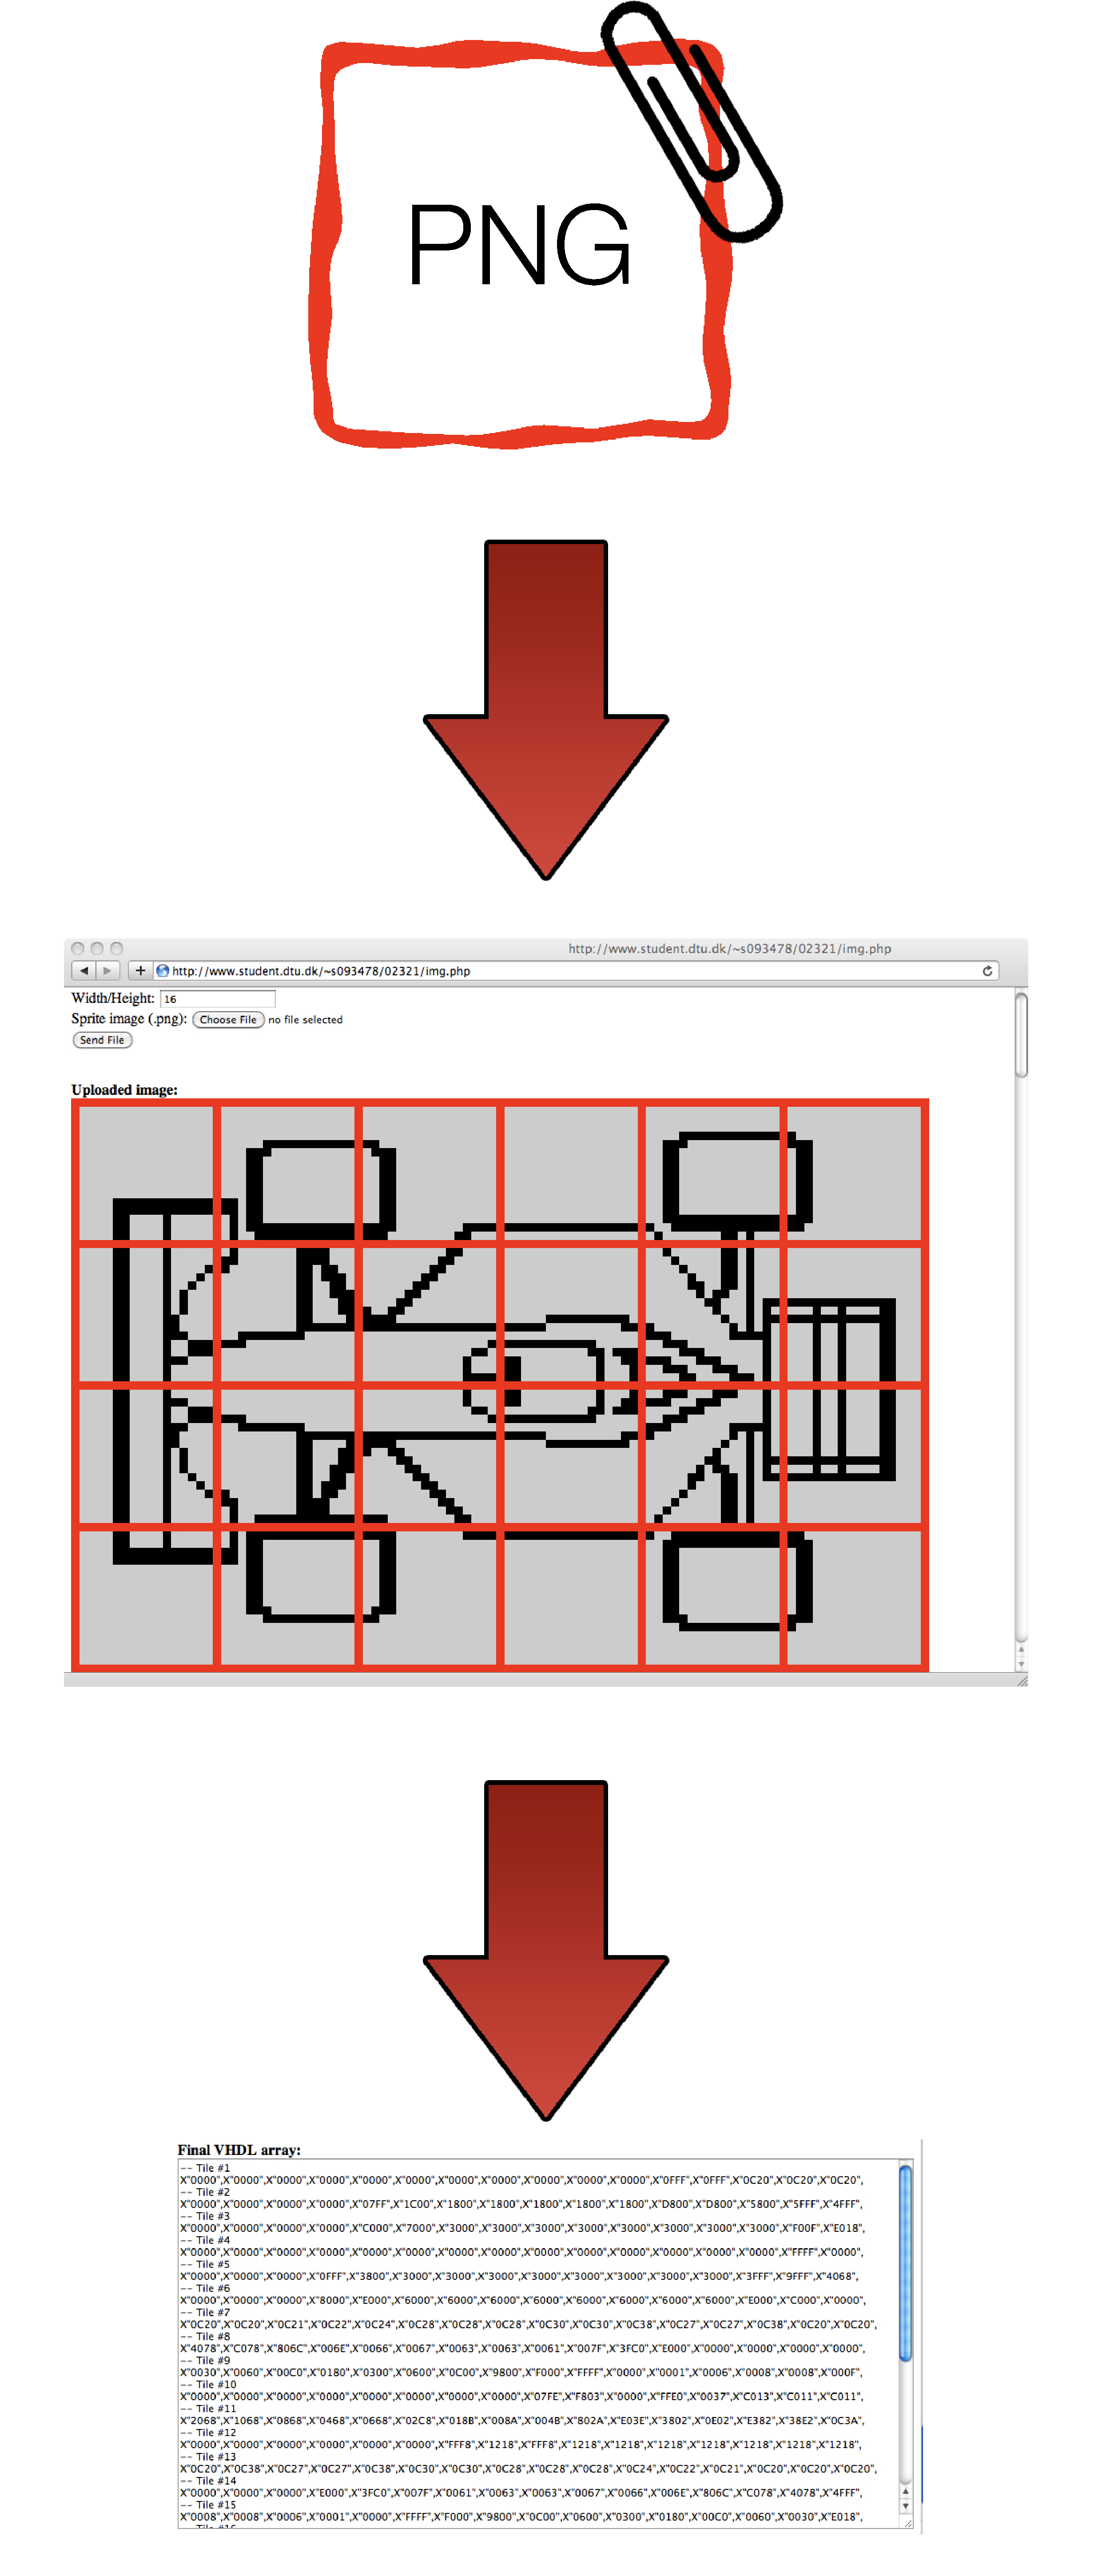
\includegraphics[width=0.28\textwidth]{billeder/SpriteMakerFlow}
  \end{center}
  \caption{Flow for oprettelse af sprites}
\end{wrapfigure}

I forbindelse med projektet er der udviklet en række online værktøjer~\cite{minitools}, hovedsageligt til at automatisere en del repetetive opgaver i forbindelse med grafik og farver til ROM.

Yderligere tekniske detaljer om udviklingen af værktøjerne er udeladt da det ikke er under formålet for projektet, ved yderligere interesse kan kildekode til alle scripts dog forefindes ved at følge kilde henvisningen.

\subsection*{Binær til VHDL array konverter}
Dette værktøj konventerer en række binære tal til et 16bit VHDL hex array, dette er f.eks. brugt til at lægge compilet assembly kode direkte i RAM på LC3'en.

\subsection*{Farve konverter}
Værktøjet konventerer en 24bit RGB farve til projektets VGA farve format som er 3 bits til rød, 3 bits til grøn og 2 bits til blå. Dette konventeres derefter til HEX så det nemt kan implementeres i VHDL.

\subsection*{Tile redigeringsværktøj}
Med tile redigeringsværktøjet er det muligt at tegne to farvede tiles direkte i browseren og generere et VHDL array således at det er muligt at ligge tile data direkte i ROM.

\subsection*{Sprite Maker}
Formålet med dette værktøj er at det er muligt at uploade en sort/hvid png fil sammen med den kvadratiske tile størrelse, derefter deler scriptet billedet op i tiles med den angivne størrelse og genererer et VHDL hex array med pixel data, sorte pixels i billede angives binært som \textbf{1} og hvide pixels angives binært som \textbf{0}.